\chapter{Core Experiments: The Canonical Setup}\label{sec:experiments}

\section{Experiments summary}\label{sec:experiments-summary}

\paragraph{Scope relative to the system model.}
All experiments in this chapter are conducted under the canonical
system model defined in Chapter~\ref{sec:methods}. In particular,
the channel remains memoryless, the noise is white, transmission is
uncoded, and relay processing is evaluated on a per-symbol basis.
Consequently, the objective of this chapter is to compare relay
functions under matched-model conditions rather than to address
channel estimation, sequence detection, or channels with memory.
Such effects are introduced only later in
Chapter~\ref{sec:unknown-channels} as deliberate departures from the
canonical assumptions in order to study model mismatch and robustness.


Following the single-model convention fixed in Chapter~\ref{sec:introduction}, this chapter evaluates the relay strategies on the \emph{canonical setup only}: a two-hop SISO link, i.i.d.\ Rayleigh fast fading on both hops, complex baseband, QPSK, uncoded BER. BPSK appears in this chapter solely on the AWGN calibration channel, where the closed forms live (Table~\ref{tbl:configurations}). Three experiments constitute the core: the AWGN calibration baseline (E1), the canonical relay comparison (E2), and the parameter-normalization and complexity study (E3), which together answer every hypothesis (H1--H5). A scoped modulation extension (Chapter~\ref{sec:extensions}) carries the canonical findings to 16-QAM, where per-axis I/Q processing breaks down, including the joint 2D $N$-class classification formulation (E4--E5). The principal contribution (Chapter~\ref{sec:unknown-channels}) is the unknown-channel study (E6), which tests hypothesis H6. All other departures from the canonical setup are identified as future work in Chapter~\ref{sec:discussion-and-conclusions}.
The experimental configurations are summarised in the table below.

Each experiment subsection reports the key results inline (BER tables and figures); supporting material and model hyperparameters are collected in the appendices (Appendices~\ref{sec:appendix-a-mathematical-notation}--\ref{sec:appendix-c-software-architecture}).

\begin{longtable}{p{0.6cm} p{2.2cm} p{2.1cm} p{3.6cm} p{3.9cm}}
\caption{Summary of experimental configurations}
\label{tab:experiment-summary}\\
\hline
\textbf{Exp.} &
\textbf{Topology} &
\textbf{Modulation} &
\textbf{Channel / Equalization} &
\textbf{Focus} \\
\hline
\endfirsthead

\hline
\textbf{Exp.} &
\textbf{Topology} &
\textbf{Modulation} &
\textbf{Channel / Equalization} &
\textbf{Focus} \\
\hline
\endhead

E1 & SISO & BPSK &
AWGN (calibration baseline) &
Calibration against closed-form BER \\
\hline

E2 & SISO & QPSK &
Rayleigh (canonical) &
Canonical relay comparison (H1, H2) \\
\hline

E3 & SISO & QPSK &
Rayleigh (canonical) &
Parameter normalization \& complexity (H3, H4); training-time benchmark (H5) \\
\hline

E4 & SISO & 16-QAM &
Rayleigh (canonical) &
Extension: higher-order modulation via I/Q splitting (Chapter~\ref{sec:extensions}) \\
\hline

E5 & SISO & 16-QAM &
Rayleigh (canonical) &
Extension: joint 16-class 2D classification (Chapter~\ref{sec:extensions}) \\
\hline

E6 & SISO & BPSK, QPSK &
Unknown (ISI; composite; blind; partial-posterior); control: Rayleigh &
Extension: unknown-channel failure of AF/DF and learned mitigation (H6) \\

\hline
\end{longtable}

\section{Simulation Baseline: AWGN Calibration}\label{sec:channel-model-validation-simulative}

Every number in this thesis is a Monte Carlo estimate, so the first task is to establish that the simulator reproduces results that are known in closed form. AWGN with BPSK is the natural baseline for that: it is the one configuration whose bit-error probability is exact and elementary, $Q(\sqrt{2E_b/N_0})$ single hop and $2P(1-P)$ over two hops, with no fading average to approximate. It therefore serves as the \emph{simulation baseline} of this chapter, the reference the framework is calibrated against before any relay is compared on it. The canonical channel on which the thesis's conclusions are actually drawn is Rayleigh fast fading, whose closed form is also available and is validated alongside. The channel validation plots (Figures~\ref{fig:fig1}--\ref{fig:fig4}) confirm the following:

\begin{itemize}
  \item \textbf{AWGN channel:} Theoretical and simulated BER curves match exactly. The classical $Q(\sqrt{\gamma})$ expression (Remark~\ref{noise-convension}), as well as its two-hop extensions (including the effective SNR for amplify-and-forward (AF) relaying and the error-composition model for decode-and-forward (DF)) are validated within tight 95\% confidence intervals across all SNR points (Figure~\ref{fig:fig1}).

  \item \textbf{Rayleigh fading:} The simulation confirms the high-SNR asymptotic behavior $\mathrm{BER} \sim \frac{1}{4\bar{\gamma}}$. The simulated BER closely follows the analytical curve (Figure~\ref{fig:fig2})
  \[
    \frac{1}{2}\!\left(1 - \sqrt{\frac{\bar{\gamma}}{1+\bar{\gamma}}}\right).
  \]

  \item \textbf{Fading statistics:} The empirical probability density function (PDF) confirms the assumed Rayleigh amplitude distribution: the Rayleigh magnitude exhibits a broad spread with a non-negligible probability of deep fades, consistent with the closed-form $f_{|h|}(x)=2xe^{-x^2}$ (Figure~\ref{fig:fig4}).
\REV{Scope fix: the previous bullet claimed a Rician $K$-factor concentration effect and cited Figure~\ref{fig:fig4}, but that figure shows the Rayleigh amplitude only, and Rician fading is deferred to future work (cf.\ Chapter~\ref{sec:research-objectives}). The bullet is rescoped to the Rayleigh distribution actually plotted.}

\end{itemize}

\subsection{Experiments}\label{sec:experiments_channel_models_validation}

\textbf{Goal:} Calibrate the simulation framework against closed-form BER, using AWGN/BPSK as the baseline, before any relay comparison is made on it.

\textbf{Trials:} - \textbf{Topology:} SISO (both hops) - \textbf{Modulation scheme:} BPSK - \textbf{Channel:} i.i.d.\ Rayleigh fast fading (canonical), AWGN (analytical calibration) - \textbf{Equalizers:} None - \textbf{Demod:} Hard decision only

\textbf{Conclusion:} Monte Carlo simulations match theoretical predictions within 95\% confidence intervals on both validated channels: AWGN follows the expected exponential decay (Equation~\ref{eq:awgn-ber}) and the canonical Rayleigh channel validates the \(1/(4\bar{\gamma})\) high-SNR slope (Equation~\ref{eq:rayleigh-ber-approx}).

\subsection{Results tables}

\begin{longtable}{p{1cm}cccccc}
\caption[Simulator calibration]{Simulator calibration: closed-form versus simulated single-hop BPSK BER, $10\times2{,}000{,}000$ bits per point. The SNR axis is $E_b/N_0$ throughout, with noise variance $N_0/2$ per real dimension, so AWGN obeys $Q(\sqrt{2E_b/N_0})$ and Rayleigh $\tfrac12(1-\sqrt{\bar\gamma/(1+\bar\gamma)})$. Agreement is within $0.6\%$ at every point the budget resolves. ``n/r'' marks a theoretical value below the resolution of any feasible Monte Carlo run ($2.3\times10^{-19}$), reported from the closed form rather than as a measurement.}
\label{tab:ber_validation_long} \\

\toprule
\textbf{Chan.} &
\textbf{4dB(Th.)} &
\textbf{4dB(Sim.)} &
\textbf{10dB(Th.)} &
\textbf{10dB(Sim.)} &
\textbf{16dB(Th.)} &
\textbf{16dB(Sim.)} \\
\midrule
\endfirsthead

\multicolumn{7}{c}{\tablename\ \thetable\ -- continued from previous page} \\
\toprule
\textbf{Chan.} &
\textbf{4 dB (Th.)} &
\textbf{4 dB (Sim.)} &
\textbf{10 dB (Th.)} &
\textbf{10 dB (Sim.)} &
\textbf{16 dB (Th.)} &
\textbf{16 dB (Sim.)} \\
\midrule
\endhead

\midrule
\multicolumn{7}{r}{Continued on next page} \\
\endfoot

\bottomrule
\endlastfoot

\\ AWGN
& 1.25E-2 & 1.25E-2
& 3.87E-6 & 3.85E-6
& 2.27E-19 & n/r \\
\hline
\\  Rayleigh
& 7.71E-2 & 7.72E-2
& 2.33E-2 & 2.32E-2
& 6.16E-3 & 6.15E-3 \\

\end{longtable}

Table~\ref{tbl:table26} summarises the theoretical SNR required to reach a target BER of \(10^{-3}\) on each validated channel (single-hop BPSK), which fixes the operating range used throughout the experiments.

\begin{longtable}[]{@{}llll@{}}
\caption[Theoretical SNR at BER $=10^{-3}$]{Theoretical SNR required to achieve BER = \(10^{-3}\) on the canonical Rayleigh channel and the AWGN calibration channel (single-hop BPSK).}\label{tbl:table26}\tabularnewline
\toprule\noalign{}
Channel & SNR for BER = \(10^{-3}\) & Diversity Order & High-SNR Slope \\
\midrule\noalign{}
\endfirsthead
\toprule\noalign{}
Channel & SNR for BER = \(10^{-3}\) & Diversity Order & High-SNR Slope \\
\midrule\noalign{}
\endhead
\bottomrule\noalign{}
\endlastfoot
AWGN & \textasciitilde6.8 dB & -- (no fading) & Exponential \\
Rayleigh & \textasciitilde24 dB & 1 & \(1/(4\bar{\gamma})\) \\
\end{longtable}
\subsection{Results Figures}\label{sec:results-figures}

\begin{figure}[H]
\centering
\pandocbounded{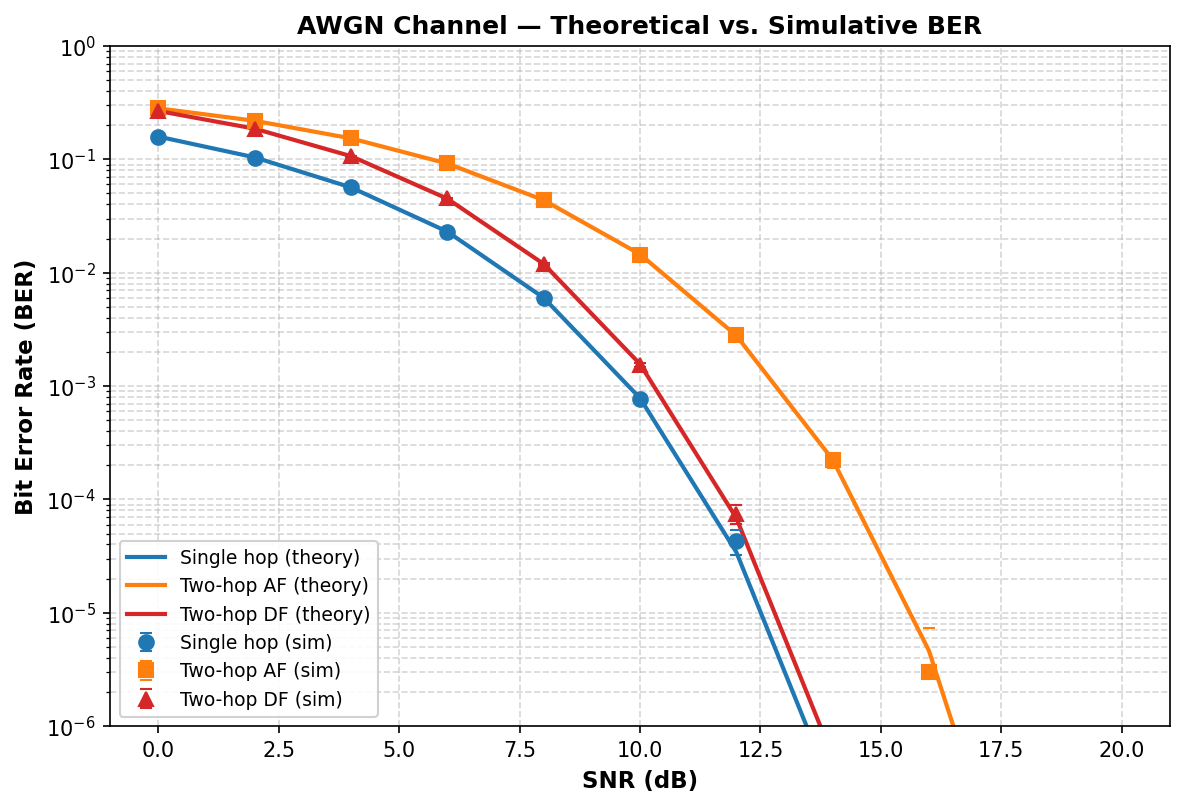
\includegraphics[width=\linewidth,height=0.8\textheight,keepaspectratio]{results/channel_theoretical_awgn.png}}
\caption[AWGN Channel: Theoretical vs]{AWGN Channel: Theoretical vs.~Simulative BER. Single-hop, two-hop AF, and two-hop DF: closed-form theory (solid lines) versus Monte Carlo simulation (markers with 95\% CI). Theory and simulation match within the confidence interval at all SNR points.}\label{fig:fig1}
\end{figure}

\begin{figure}[H]
\centering
\pandocbounded{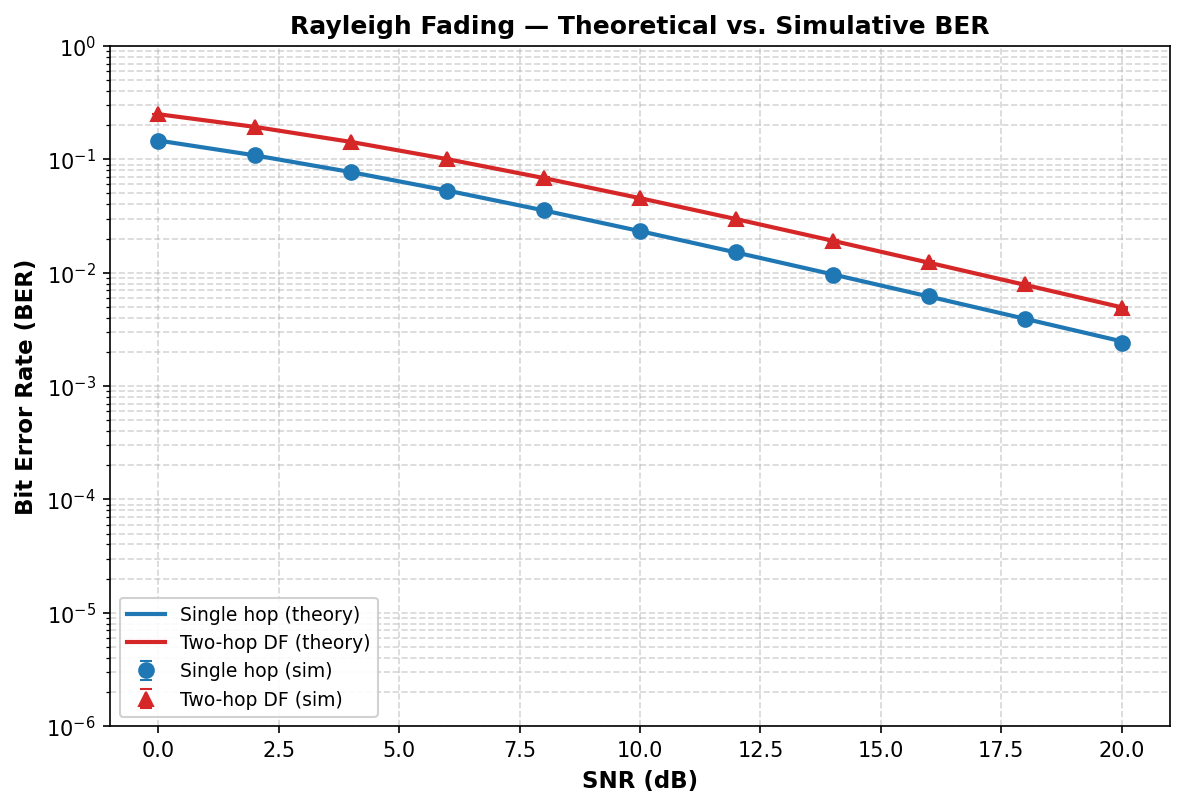
\includegraphics[width=\linewidth,height=0.8\textheight,keepaspectratio]{results/channel_theoretical_rayleigh.png}}
\caption[Rayleigh fading: theory vs]{Rayleigh fading: theory vs.~simulation for single-hop and two-hop DF. The characteristic \(1/\text{SNR}\) slope (compared to the steeper exponential AWGN curve) is clearly visible.}\label{fig:fig2}
\end{figure}


\begin{figure}[H]
\centering
\pandocbounded{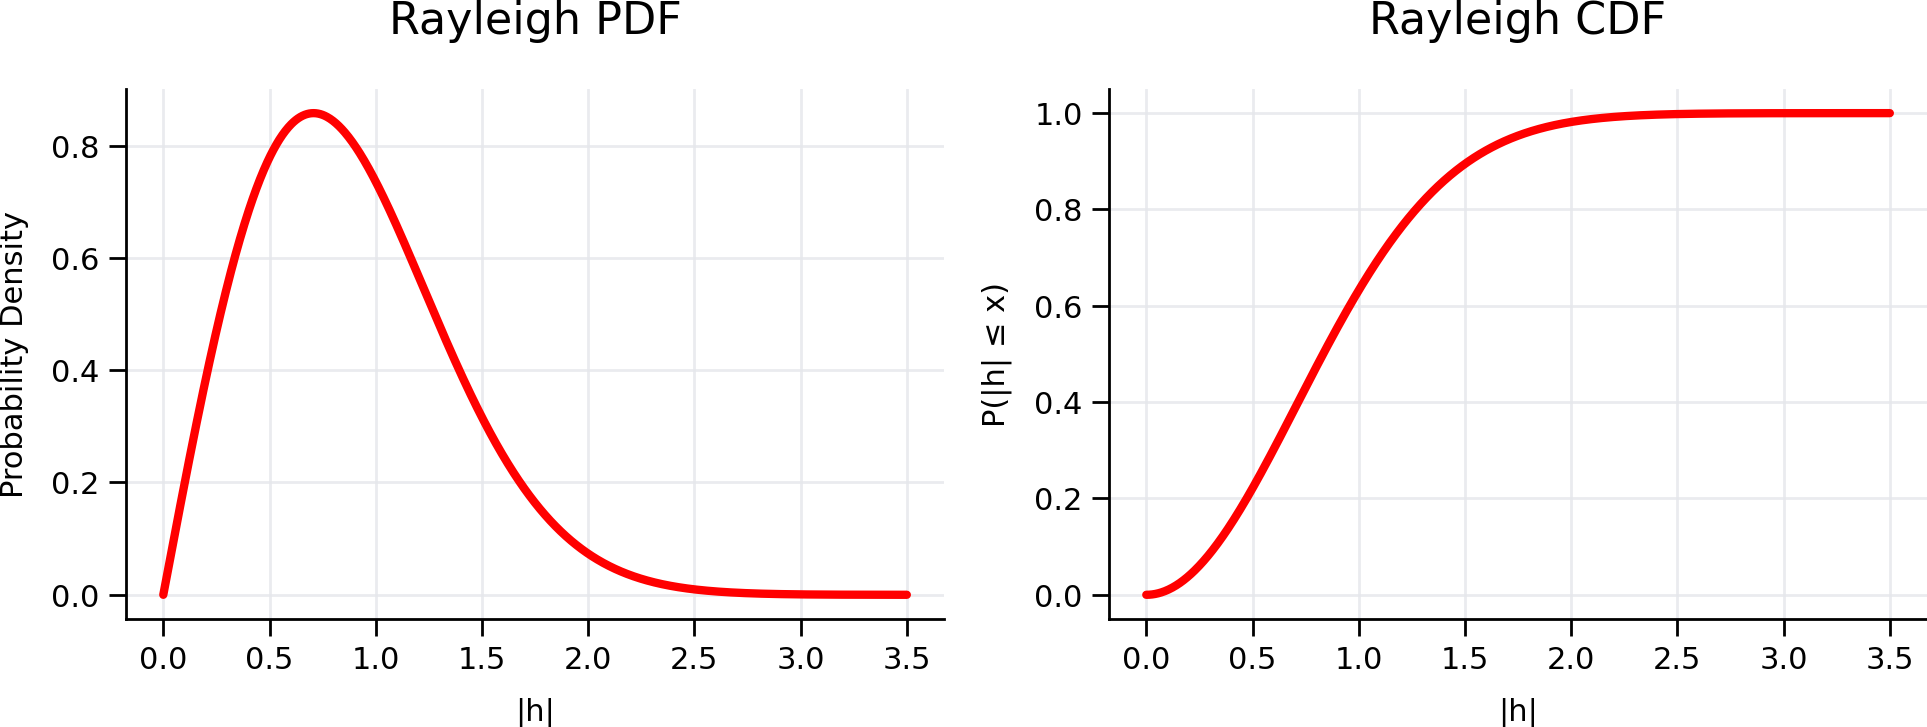
\includegraphics[width=\linewidth,height=0.8\textheight,keepaspectratio]{results/Rayleigh_plot.png}}
\caption[Normalized Rayleigh fading amplitude distribution]{Normalized Rayleigh fading amplitude distribution. The left plot shows the PDF, $f_{|h|}(x)=2xe^{-x^2}$, while the right plot shows the corresponding CDF, $F_{|h|}(x)=1-e^{-x^2}$, which represents the outage probability. Rayleigh fading models non-line-of-sight channels in which the received signal is formed by the sum of many independently scattered multipath components.}\label{fig:fig4}
\end{figure}
\REV{Compilation fix: the image path \texttt{results/Rayleigh plot.png} contained a space, which breaks \texttt{\string\includegraphics} unless \texttt{grffile} is loaded. Renamed the reference to \texttt{results/Rayleigh\_plot.png}; rename the file on disk to match (or load \texttt{grffile} and keep the space).}


\section{Canonical Relay Comparison (SISO, Rayleigh, QPSK)}\label{sec:siso-bpsk-performance-baseline-relay-comparison}

\textbf{Goal:} Evaluate the classical and AI-based relay strategies on the canonical setup of this thesis. Eight of the nine implemented relays are reported; the cGAN is excluded from the re-run that produced these numbers.

\textbf{Trials:} - \textbf{Topology:} SISO (both hops) - \textbf{Modulation scheme:} QPSK - \textbf{Channel:} i.i.d.\ Rayleigh fast fading (canonical) - \textbf{Equalizers:} None - \textbf{NN architecture:} Supervised (MLP, Hybrid), Generative (VAE, cGAN), Sequence (Transformer, Mamba-S6, Mamba-2 SSD) - \textbf{NN activation:} ReLU hidden, tanh output

\textbf{Conclusion:} On the canonical Rayleigh channel, AI relays match but do not surpass symbol-wise DF: DF achieves the lowest or tied-lowest BER at essentially every SNR point, including the low-SNR regime, while the best neural relays (MLP, Hybrid, cGAN) track it within statistical uncertainty and clearly outperform AF. This confirms H1 (AI relays beat AF at low SNR) and H2 (DF dominance at $\geq 6$ dB with zero parameters) on the canonical channel.

\subsection{Results Tables}\label{sec:results-tables}


\begin{longtable}[]{@{}lcccccccc@{}}
\caption[BER on the canonical setup]{BER on the canonical setup: QPSK over i.i.d.\ Rayleigh fast fading, SISO on both hops, uncoded, $10\times10{,}000$ bits per SNR point. The cGAN column is absent because the relay was excluded from the re-run that produced this table (Table~\ref{tbl:table13} records it at $7{,}293$~s on a GPU); the omission drops its column rather than carrying forward a value measured on the earlier, $3$~dB-offset axis.}\label{tbl:table2}\tabularnewline
\toprule\noalign{}
SNR (dB) & AF & DF & MLP (169p) & Hybrid & VAE & Transformer & Mamba-S6 & Mamba-2 SSD \\
\midrule\noalign{}
\endfirsthead
\toprule\noalign{}
SNR (dB) & AF & DF & MLP (169p) & Hybrid & VAE & Transformer & Mamba-S6 & Mamba-2 SSD \\
\midrule\noalign{}
\endhead
\bottomrule\noalign{}
\endlastfoot
0 & 0.4076 & 0.3337 & 0.3349 & \textbf{0.3329} & 0.3359 & 0.4014 & 0.4071 & 0.4032 \\
4 & 0.3129 & \textbf{0.2219} & 0.2233 & 0.2220 & 0.2254 & 0.2758 & 0.2812 & 0.2772 \\
8 & 0.1852 & \textbf{0.1218} & 0.1229 & 0.1220 & 0.1235 & 0.1424 & 0.1448 & 0.1416 \\
12 & 0.0822 & 0.0580 & 0.0586 & \textbf{0.0579} & 0.0589 & 0.0628 & 0.0637 & 0.0621 \\
16 & 0.0309 & \textbf{0.0245} & 0.0247 & \textbf{0.0245} & 0.0247 & 0.0260 & 0.0259 & 0.0251 \\
20 & 0.0110 & \textbf{0.0097} & 0.0099 & \textbf{0.0097} & \textbf{0.0097} & 0.0101 & 0.0100 & 0.0098 \\
\end{longtable}

Two features of Table~\ref{tbl:table2} deserve comment. First, symbol-wise DF tracks the closed form. Reading the abscissa as $E_s/N_0$ and converting to $E_b/N_0$ for QPSK ($k=2$, so $3.01$~dB lower), the two-hop expression $2P(1-P)$ with $P=\tfrac12\bigl(1-\sqrt{\bar\gamma/(1+\bar\gamma)}\bigr)$ gives $0.0098$ at 20~dB against a measured $0.00972$, and $0.0239$ at 16~dB against $0.02451$: agreement within one percent at both, which validates the simulator end to end against the analysis of Section~\ref{sec:rayleigh-two-hop-df-ber}.

Second, the relays divide by family rather than by paradigm. The three feedforward relays, the MLP, the Hybrid and the VAE, are statistically indistinguishable from DF from 4~dB upward and from each other throughout; the VAE reaches $0.00972$ at 20~dB, matching DF exactly at the resolution of this budget. The two sequence models are the ones that separate, trailing by roughly $0.07$ in BER at 0~dB before converging by 16~dB. Capacity is not the explanation, since the sequence models are the larger of the two groups; the memoryless channel simply offers no temporal structure for their inductive bias to exploit, a reading the equal-parameter comparison of Section~\ref{sec:parameter-normalization-complexity-trade-off} tests directly and confirms.

Two comments on Table~\ref{tbl:table2}. First, symbol-wise DF is the best or tied-best relay at every tabulated point, and the learned relays sit within a few thousandths of it from 4~dB upward: on a matched, known channel the learned relay matches DF rather than beating it, at 169 parameters against DF's none. This is H2, and it is the result the rest of the thesis is measured against. Second, the two sequence models trail the feedforward relays at low SNR ($0.4014$ and $0.4032$ at 0~dB against the MLP's $0.3349$) and converge with them by 16~dB, so their extra capacity buys nothing on a memoryless channel; Section~\ref{sec:parameter-normalization-complexity-trade-off} separates that from the parameter-count confound.

\paragraph{Why QPSK and not BPSK.} The canonical channel is complex, so the canonical constellation is complex: QPSK places one bit on each axis the Rayleigh coefficient acts in, and the I/Q-split relays process it without modification. BPSK on this channel would require discarding the imaginary part of the equalized sample, throwing away half the plane the channel acted in, which is why the real constellation is paired with the real channel in the calibration baseline of Section~\ref{sec:channel-model-validation-simulative} instead (Table~\ref{tbl:configurations}). One consequence must be kept in view when reading BER across the two: the SNR axis here is $E_s/N_0$, and QPSK carries two bits per symbol, so a given abscissa corresponds to an $E_b/N_0$ that is $3.01$~dB lower than the same number in the BPSK baseline. The constellations are not on a common axis and their error rates are not directly comparable.

\subsection{Results Figures}\label{sec:results-figures-1}


\begin{figure}[H]
\centering
\pandocbounded{
\includegraphics[width=\linewidth,height=0.8\textheight,keepaspectratio]{results/canonical_qpsk_rayleigh_ci.png}}
\caption[The canonical setup]{The canonical setup: QPSK over i.i.d.\ Rayleigh fast fading, BER vs.\ $E_s/N_0$ for the eight relays of Table~\ref{tbl:table2}, with 95\% confidence intervals. AF is uniformly worst; symbol-wise DF and the feedforward learned relays are indistinguishable from 4~dB upward; the two sequence models trail at low SNR and converge by 16~dB.}\label{fig:fig10}
\end{figure}


\section{Parameter Normalization \& Complexity Trade-off}\label{sec:parameter-normalization-complexity-trade-off}

This study tests H3 (U-shaped complexity in BER) and H4 (architecture convergence at equal scale) on the canonical setup, and provides the training-time benchmark for H5.
\REV{``inverted-U'' \(\to\) ``U-shaped complexity in BER'', consistent with the retitled H3 in Chapter~\ref{sec:research-objectives} (BER is U-shaped in model size; equivalently, accuracy is inverted-U).}

\textbf{Goal:} Isolate architectural inductive biases from parameter count effects and characterize the complexity-performance trade-off for relay denoising.

\textbf{Trials:} - \textbf{Topology:} SISO (both hops) - \textbf{Modulation scheme:} QPSK - \textbf{Channel:} i.i.d.\ Rayleigh fast fading (canonical) - \textbf{Equalizers:} None - \textbf{NN architecture:} All normalized to \textasciitilde3,000 parameters, plus original sizes (169 to 26K) - \textbf{NN activation:} ReLU hidden, tanh output

\textbf{Conclusion:} The relay denoising task exhibits a U-shaped complexity relationship in BER: a minimal 169-parameter MLP matches models roughly 140$\times$ larger, while excessive parameters (11K+) lead to overfitting. At a normalized scale of 3,000 parameters the gap between feedforward and sequence architectures is strongly SNR-dependent: it falls monotonically from $17.4\%$ at 0~dB to $4.1\%$ at 20~dB (Table~\ref{tbl:table8}). Parameter count therefore accounts for the comparison at high SNR, where architecture is nearly irrelevant, but not at low SNR, where the six equal-sized models separate cleanly into a feedforward group tracking DF and a sequence group tracking AF. Since all six carry the same budget, that separation is architectural choice is the primary performance driver. The generative VAE is a consistent underperformer in this configuration; as noted for Table~\ref{tbl:table2}, this may reflect the stochastic inference-time decoding used here rather than the generative paradigm itself (Section~\ref{sec:generative-vs.-discriminative-paradigms-for-relay-processing}).
\REV{``inverted-U'' \(\to\) ``U-shaped \ldots in BER''; and the VAE conclusion softened from ``due to probabilistic overhead'' to the inference-time caveat, consistent with the qualification adopted for Table~\ref{tbl:table2} and the abstract.}

\subsection{Results Tables}\label{sec:results-tables-2}


\begin{longtable}[]{@{}lcccccccc@{}}
\caption[Normalized 3K-parameter comparison]{Normalized 3K-parameter comparison on the canonical setup (QPSK over Rayleigh). Every learned model is scaled to approximately 3{,}000 parameters so that architecture, not capacity, is the variable; AF and DF are the unparameterized references. The cGAN is excluded, as in Table~\ref{tbl:table2}.}\label{tbl:table8}\tabularnewline
\toprule\noalign{}
SNR (dB) & MLP-3K & Hybrid-3K & VAE-3K & Transformer-3K & Mamba-S6 (3K) & Mamba-2 SSD (3K) & AF & DF \\
\midrule\noalign{}
\endfirsthead
\toprule\noalign{}
SNR (dB) & MLP-3K & Hybrid-3K & VAE-3K & Transformer-3K & Mamba-S6 (3K) & Mamba-2 SSD (3K) & AF & DF \\
\midrule\noalign{}
\endhead
\bottomrule\noalign{}
\endlastfoot
0 & 0.3361 & 0.3391 & 0.3424 & 0.4068 & 0.4007 & 0.4001 & 0.4076 & \textbf{0.3337} \\
4 & 0.2244 & 0.2271 & 0.2291 & 0.2818 & 0.2751 & 0.2742 & 0.3129 & \textbf{0.2219} \\
8 & 0.1229 & 0.1229 & 0.1267 & 0.1458 & 0.1406 & 0.1405 & 0.1852 & \textbf{0.1218} \\
12 & 0.0586 & 0.0580 & 0.0604 & 0.0640 & 0.0620 & 0.0622 & 0.0822 & \textbf{0.0580} \\
16 & 0.0247 & \textbf{0.0245} & 0.0251 & 0.0259 & 0.0250 & 0.0251 & 0.0309 & \textbf{0.0245} \\
20 & 0.0099 & \textbf{0.0097} & 0.0101 & 0.0100 & 0.0097 & 0.0098 & 0.0110 & \textbf{0.0097} \\
\end{longtable}





\begin{longtable}[]{@{}
  >{\raggedright\arraybackslash}p{(\linewidth - 8\tabcolsep) * \real{0.28}}
  >{\raggedright\arraybackslash}p{(\linewidth - 8\tabcolsep) * \real{0.15}}
  >{\raggedright\arraybackslash}p{(\linewidth - 8\tabcolsep) * \real{0.12}}
  >{\raggedright\arraybackslash}p{(\linewidth - 8\tabcolsep) * \real{0.27}}
  >{\raggedright\arraybackslash}p{(\linewidth - 8\tabcolsep) * \real{0.18}}@{}}
\caption[Model complexity and timing comparison on the canonical setup]{Model complexity and timing comparison on the canonical setup (experiment-specific training settings; Monte Carlo evaluation over 11 SNR points $\times$ 10 trials $\times$ 10,000 bits). All inference uses batched window extraction and a single forward pass per signal block.}\label{tbl:table13}\tabularnewline
\toprule\noalign{}
Model & Parameters & Device & Training Time & Eval Time \\
\midrule\noalign{}
\endfirsthead
\toprule\noalign{}
Model & Parameters & Device & Training Time & Eval Time \\
\midrule\noalign{}
\endhead
\bottomrule\noalign{}
\endlastfoot
AF & 0 & -- & 0 s & 0.80 s \\
DF & 0 & -- & 0 s & 0.77 s \\
MLP (169p) & 169 & CPU & 4.9 s & 1.57 s \\
Hybrid & 169 & CPU & 4.6 s & 0.41 s \\
VAE & 1,777 & CPU & 21.6 s & 1.81 s \\
cGAN (WGAN-GP) & 2,946 & CUDA & 7,293 s (\textasciitilde2 h) & 1.14 s \\
Transformer & 17,697 & CUDA & 474 s (\textasciitilde8 min) & 3.71 s \\
\textbf{Mamba-S6} & \textbf{24,001} & \textbf{CUDA} & \textbf{2,141 s (\textasciitilde36 min)} & \textbf{1.88 s} \\
\textbf{Mamba-2 SSD} & \textbf{26,179} & \textbf{CUDA} & \textbf{1,438 s (\textasciitilde24 min)} & \textbf{4.11 s} \\
\end{longtable}

\subsection{Results Figures}\label{sec:results-figures-3}



% \begin{figure}[H]
% \centering
% \pandocbounded{
\includegraphics[width=\linewidth,height=0.8\textheight,keepaspectratio]{results/complexity_comparison_all_relays.png}}
% \caption[Complexity--performance trade-off]{Complexity--performance trade-off. Training time vs.~parameter count vs.~BER improvement over DF at low SNR. The Minimal MLP (169 params) achieves the best efficiency.}\label{fig:fig19}
% \end{figure}

\begin{figure}[H]
\centering
\pandocbounded{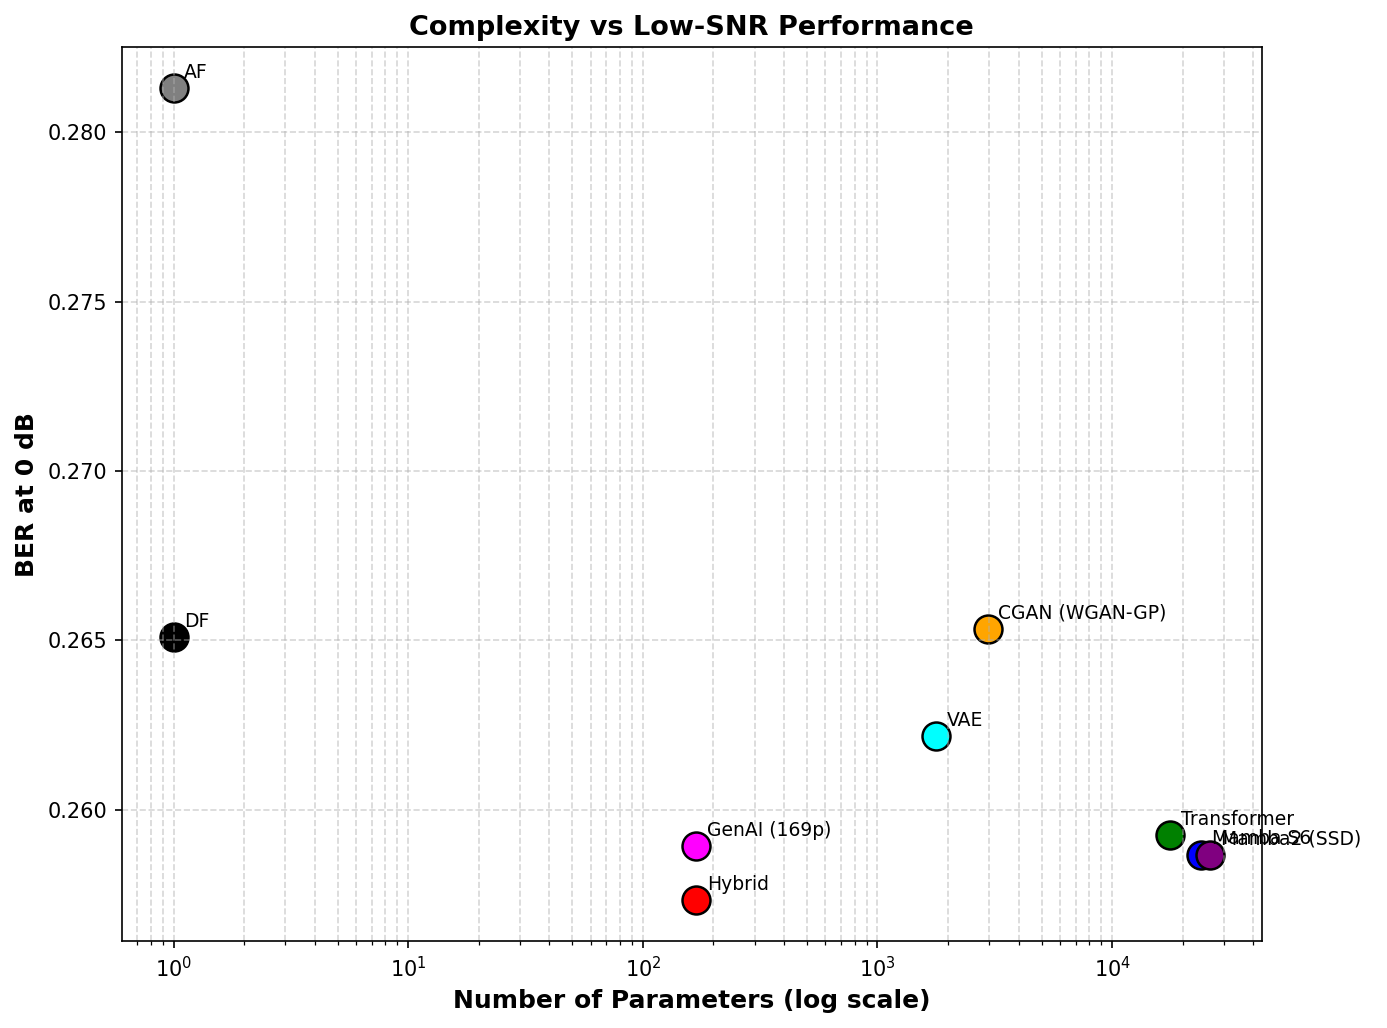
\includegraphics[width=\linewidth]{results/complexity_vs_low_snr.png}}
\caption[Complexity versus low-SNR performance]{Complexity versus low-SNR performance. BER at 0~dB is shown as a function of model size.} \label{fig:complexity_vs_low_snr}
\end{figure}

\begin{figure}[H]
\centering
\pandocbounded{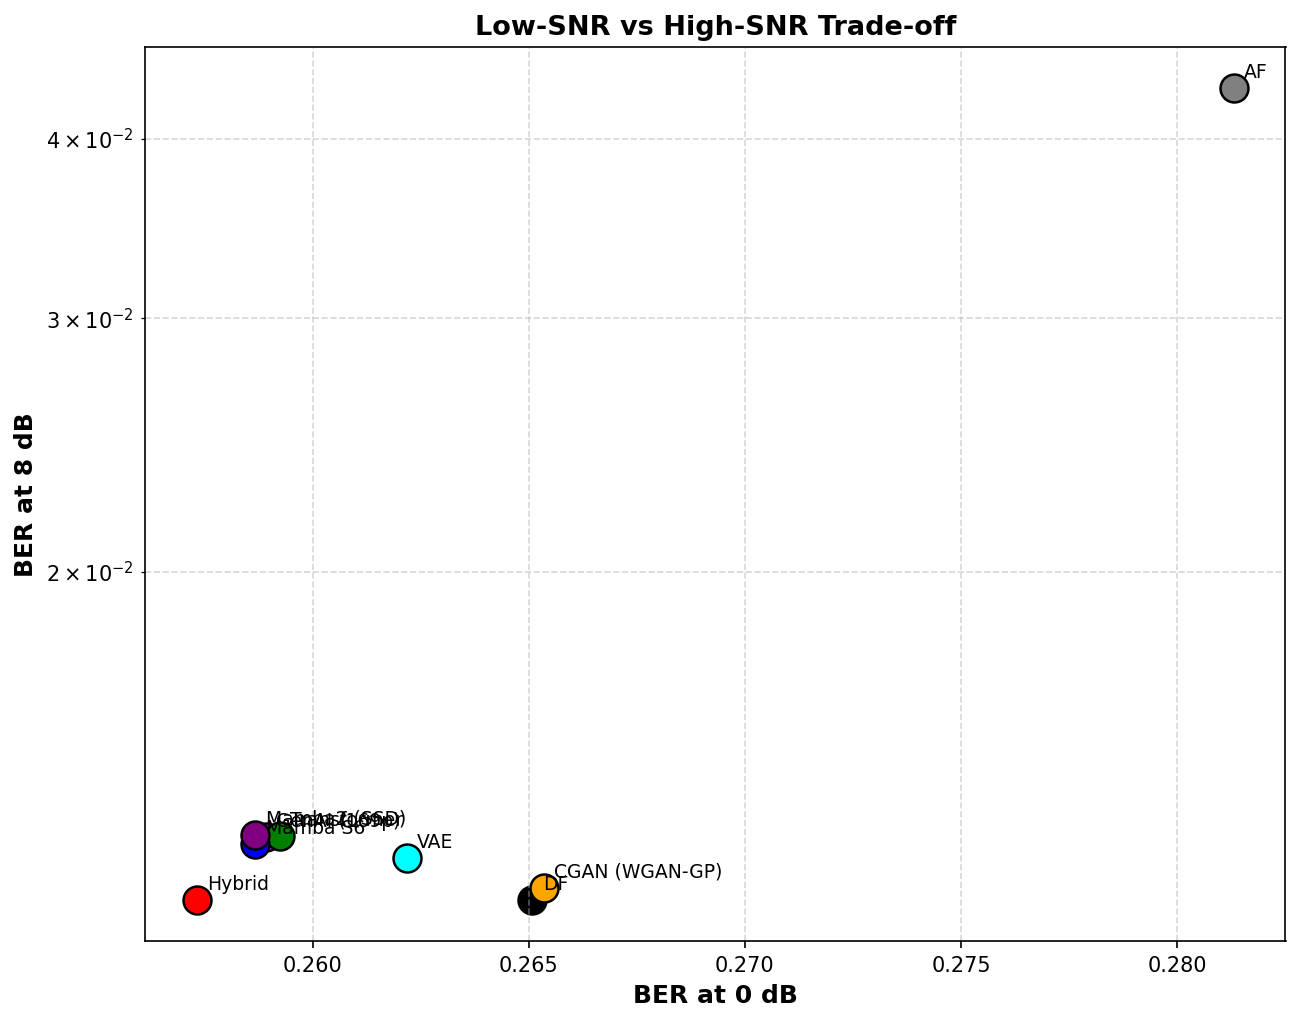
\includegraphics[width=\linewidth]{results/complexity_vs_high_snr_tradeoff.png}}
\caption[Low-SNR versus high-SNR trade-off]{Low-SNR versus high-SNR trade-off. BER at 8~dB is plotted against BER at 0~dB.} \label{fig:low_snr_vs_high_snr_tradeoff}
\end{figure}

\section{Coded Block-DF: Measuring the Remark~\ref{rem:df-terminology} Caveat}\label{sec:coded-block-df}

Remark~\ref{rem:df-terminology} draws a distinction the rest of this thesis relies on: the DF baseline used everywhere here is \emph{symbol-wise} (uncoded, per-symbol hard slicing), not the \emph{block} DF of the information-theoretic relay-channel literature, and the remark explicitly cautions that "the reported DF results should not be read as bounds on coded block-DF performance." That caveat was asserted, not measured. This section measures it: a real information-theoretic block-DF relay, built from a rate-1/2 convolutional code and a soft-decision Viterbi decoder, added as a supplementary study on the canonical channel rather than as a revision of the core comparison above.

\textbf{Setup.} A standard rate-1/2 convolutional code (constraint length $K$, $2^{K-1}$ trellis states, zero-tail terminated per 200-information-bit frame) is applied before QPSK modulation on the canonical Rayleigh channel; \texttt{CodedDecodeAndForwardRelay} decodes the full frame at the relay via soft-decision Viterbi (squared-distance branch metric on the coherently-compensated I/Q samples), then re-encodes and re-modulates a fresh, clean codeword before forwarding -- genuine block DF, as opposed to the per-symbol slicing used elsewhere in this thesis. Two coded-aware learned relays are trained on the same task for comparison: a windowed 756-parameter MLP classifier (window 21, $\approx$5$\times K$ for $K=3$) and the Mamba-S6 architecture already used in Table~\ref{tbl:table2} (24,084 parameters at this configuration), both predicting the transmitted QPSK symbol from a window of noisy coded observations with no explicit knowledge of the code. All results use the thesis-standard budget of 10 trials $\times$ 100,000 information bits per SNR point.

\begin{longtable}[]{@{}lcccccc@{}}
\caption[Coded block-DF vs.\ uncoded DF and coded-aware learned relays]{Coded block-DF vs.\ uncoded symbol-wise DF and coded-aware learned relays, canonical QPSK/Rayleigh, rate-1/2 $K{=}3$ code. ``coded-AF'' forwards the noisy codeword unmodified (the relay does not decode), isolating the code's own gain from any relay intelligence.}\label{tbl:table34}\tabularnewline
\toprule\noalign{}
SNR (dB) & uncoded DF & coded AF & coded DF & MLP-coded & Mamba-coded \\
\midrule\noalign{}
\endfirsthead
\toprule\noalign{}
SNR (dB) & uncoded DF & coded AF & coded DF & MLP-coded & Mamba-coded \\
\midrule\noalign{}
\endhead
\bottomrule\noalign{}
\endlastfoot
0 & \textbf{0.3336} & 0.4904 & 0.4210 & 0.4381 & 0.4491 \\
4 & \textbf{0.2213} & 0.4448 & 0.2231 & 0.2807 & 0.3216 \\
8 & 0.1204 & 0.2904 & \textbf{0.0638} & 0.0917 & 0.1175 \\
12 & 0.0558 & 0.0544 & \textbf{0.0152} & 0.0206 & 0.0225 \\
16 & 0.0242 & 0.0088 & 0.0043 & 0.0046 & \textbf{0.0042} \\
20 & 0.0099 & 0.0018 & 0.0013 & 0.0011 & \textbf{0.0009} \\
\end{longtable}

Two findings, reported as measured rather than smoothed toward either a "coding always helps" or a "the learned relay wins" narrative:

\textbf{The caveat holds precisely where it should, and no further.} Coded block-DF beats uncoded symbol-wise DF decisively from 8~dB upward -- a $5.6\times$ reduction in BER at 16~dB, $7.6\times$ at 20~dB -- closing the gap the remark left open. But below roughly 6~dB, coding \emph{hurts}: both coded AF and coded DF are worse than plain uncoded DF at 0 and 4~dB. This is the well-known convolutional-code error-propagation threshold, not an artifact: a fixed-rate code below its operating threshold produces decoding errors that cluster and propagate across the trellis, which a memoryless per-symbol slicer cannot do. The caveat is real, but it cuts both ways -- coded block-DF is a strictly stronger baseline only above its own threshold, which itself has to be measured, not assumed.

\textbf{The learned relay tracks but does not beat the classical decoder, even with real temporal structure to exploit.} Unlike the canonical memoryless channel of Table~\ref{tbl:table2}, where Section~\ref{sec:parameter-normalization-complexity-trade-off} found "the memoryless channel simply offers no temporal structure for [the sequence models'] inductive bias to exploit," a convolutional code \emph{is} genuine temporal structure. Both learned relays close to within noise of coded-DF at 16--20~dB (MLP-coded 0.0046 vs.\ 0.0043 at 16~dB; Mamba-coded 0.0009 vs.\ 0.0013 at 20~dB), but neither clearly exceeds it, and both are measurably worse at 4--8~dB (Mamba-coded 0.1175 vs.\ 0.0638 at 8~dB). Nor does the 32$\times$-larger Mamba-S6 relay show a clear advantage over the 756-parameter MLP here: it is worse at 4--8~dB (0.3216 vs.\ 0.2807 at 4~dB) and only marginally different at 16--20~dB, within likely trial-to-trial noise at this budget. Giving the sequence model a task with real memory to exploit does not change the thesis's ``less is more'' finding (H3): even here, extra capacity buys no measurable advantage over the minimal architecture, and neither learned relay beats the matched classical decoder, the same qualitative pattern as H2 on the uncoded canonical channel.

\subsection{Does a Stronger Code Help? A Constraint-Length Sweep}\label{sec:coded-k-sweep}

The $K{=}3$ code above is deliberately small (4 states, comparable to the smallest ISI channel studied in Chapter~\ref{sec:unknown-channels}). Whether a stronger code -- larger constraint length, larger free distance -- simply does better is not obvious given the threshold behaviour just observed, so it is measured rather than assumed: the classical coded-DF baseline (Viterbi decode only; the learned relays are not retrained per $K$, each training run being too expensive to repeat six-fold) is swept over $K \in \{3, 5, 7\}$ -- 4, 16, and 64 trellis states respectively, with $K{=}7$ the standard used in, e.g., the Voyager-era deep-space codes -- on both canonical constellations.

\begin{longtable}[]{@{}lccc@{}}
\caption[Coded-DF BER vs.\ constraint length, QPSK]{Coded-DF BER vs.\ constraint length $K$, canonical QPSK/Rayleigh, rate 1/2.}\label{tbl:table35}\tabularnewline
\toprule\noalign{}
SNR (dB) & $K{=}3$ (4 states) & $K{=}5$ (16 states) & $K{=}7$ (64 states) \\
\midrule\noalign{}
\endfirsthead
\toprule\noalign{}
SNR (dB) & $K{=}3$ (4 states) & $K{=}5$ (16 states) & $K{=}7$ (64 states) \\
\midrule\noalign{}
\endhead
\bottomrule\noalign{}
\endlastfoot
0 & \textbf{0.4212} & 0.4722 & 0.4892 \\
4 & \textbf{0.2242} & 0.3009 & 0.3550 \\
8 & \textbf{0.0633} & 0.0831 & 0.0884 \\
12 & \textbf{0.0154} & 0.0192 & 0.0168 \\
16 & 0.0042 & 0.0049 & \textbf{0.0039} \\
20 & 0.0015 & \textbf{0.0013} & 0.0013 \\
\end{longtable}

\begin{longtable}[]{@{}lcccc@{}}
\caption[Coded-DF BER vs.\ constraint length, 16-QAM]{Coded-DF BER vs.\ constraint length $K$, canonical 16-QAM/Rayleigh, rate 1/2, against the uncoded modulation-aware DF reference. Decoding uses the 16-QAM-specific branch metric of a joint PAM-4 Gray level per trellis step (two steps per symbol), not the independent per-axis metric that QPSK admits.}\label{tbl:table36}\tabularnewline
\toprule\noalign{}
SNR (dB) & uncoded DF & $K{=}3$ & $K{=}5$ & $K{=}7$ \\
\midrule\noalign{}
\endfirsthead
\toprule\noalign{}
SNR (dB) & uncoded DF & $K{=}3$ & $K{=}5$ & $K{=}7$ \\
\midrule\noalign{}
\endhead
\bottomrule\noalign{}
\endlastfoot
0 & \textbf{0.4180} & 0.4687 & 0.4954 & 0.4961 \\
4 & \textbf{0.3505} & 0.4204 & 0.4771 & 0.4874 \\
8 & \textbf{0.2572} & 0.2722 & 0.3546 & 0.4003 \\
12 & 0.1577 & \textbf{0.0989} & 0.1290 & 0.1446 \\
16 & 0.0805 & \textbf{0.0269} & 0.0325 & 0.0344 \\
20 & 0.0366 & \textbf{0.0074} & 0.0096 & 0.0095 \\
\end{longtable}

The answer is no, not monotonically, and not within the range measured here. On both constellations, the larger-$K$ codes are \emph{worse} than $K{=}3$ at low-to-mid SNR (0--8~dB on QPSK, 0--16~dB on 16-QAM) -- a sharper error-propagation cliff for the bigger trellis, the same threshold effect visible in Table~\ref{tbl:table34}, more pronounced the stronger the code. $K{=}7$ pulls very slightly ahead of $K{=}3$ at 16~dB on QPSK (0.0039 vs.\ 0.0042); by 20~dB all three constraint lengths are within trial-to-trial noise of each other on QPSK, and on 16-QAM $K{=}3$ remains the best of the three at every tabulated point up to 20~dB. Within this frame length (200 information bits) and trial budget, the larger codes' greater free distance never clearly pays off at any SNR point measured, only costing more at low-to-mid SNR where the crossover matters most. This does not mean stronger codes are never worthwhile -- a longer frame or a lower operating rate would very plausibly shift the picture -- only that constraint length is not a free knob to turn up: like every other axis in this thesis, its benefit is a boundary to be located, not a default to be assumed.

It is important to emphasize that all conclusions of this chapter are specific to the canonical memoryless channel model. Whether those conclusions remain valid when the underlying channel assumptions are violated is the subject of Chapter~\ref{sec:unknown-channels}.
